\documentclass[12pt]{beamer}
\usetheme{Boadilla}
\usepackage{booktabs}
\usepackage{multirow}
\usepackage{enumitem}
\usepackage{tikz}

\newcommand{\E}{\mathbb{E}}
\usefonttheme{professionalfonts}
\usepackage{pgfplots}
\pgfplotsset{compat=1.18}
\renewcommand{\arraystretch}{1.25}
\usetikzlibrary{trees}
\title[ECON2843]{Lecture 19}
\subtitle{Part 4 Analysis of Variance}
\date{}
\usepackage{amsmath,amssymb,mathtools,wasysym}
\begin{document}
	\begin{frame}
		\titlepage
	\end{frame}
	\begin{frame}
		\vspace{1cm}
		\centering
		{\color{blue}\large Two-way ANOVA}
	\end{frame}
\begin{frame}
	\frametitle{Two-way ANOVA}
	
	\begin{itemize}[label={\color{blue}$\blacktriangleright$}]
		\item In a two-way ANOVA, we have:
		\begin{itemize}[label={\color{blue}$\blacktriangleright$}]
			\item One continuous response variable $Y$.
			\item Two categorical variables (factors), each with a potentially different number of categories (levels).
			\item Each factor must still have at least two levels.
		\end{itemize}
		\item For a two-way ANOVA, a particular combination of levels from the two factors is called a \textbf{treatment} and represents a population.
	\end{itemize}
	
\end{frame}
	\begin{frame}
		\frametitle{Treatment}
		
		\begin{itemize}[label={\color{blue}$\blacktriangleright$}]
			\item Suppose our two factors, denoted $A$ and $B$, have three levels $(A_1, A_2, A_3)$ and two levels $(B_1, B_2)$, respectively.
			\item There are $3 \times 2 = 6$ treatments, as shown below:
		\end{itemize}
		
		\vspace{0.5cm}
		
		\begin{center}
			\begin{tabular}{ccc}
				\toprule
				Treatment & \multicolumn{2}{c}{Levels} \\
				\midrule
				1 & $A_1$ & $B_1$ \\
				2 & $A_1$ & $B_2$ \\
				3 & $A_2$ & $B_1$ \\
				4 & $A_2$ & $B_2$ \\
				5 & $A_3$ & $B_1$ \\
				6 & $A_3$ & $B_2$ \\
				\bottomrule
			\end{tabular}
		\end{center}
		
	\end{frame}
	\begin{frame}
		\frametitle{Terminology}
		
		\begin{itemize}[label={\color{blue}$\blacktriangleright$}]
			\item A \textbf{complete factorial experiment} is one where sample data is collected for every possible combination of levels of the two factors. That is, we have data for all treatments.
			
			\item A complete factorial experiment is \textbf{balanced} if the number of observations collected for each treatment (also called \textbf{replicates}) is the same.
			
			\item In the example on the previous slide, if we collected, e.g., five replicates for each of the six treatments, we would have a balanced two-way ANOVA.
		\end{itemize}
		
	\end{frame}
	\begin{frame}
		\frametitle{Assumptions}
		
		\begin{itemize}[label={\color{blue}$\blacktriangleright$}]
			\item We must also make some assumptions when performing a two-way ANOVA:
		\end{itemize}
		
		
		\begin{enumerate}[label=\textcolor{blue}{\arabic*.}]
			\item The levels of both factors are fixed beforehand.
			\item The response variable is normally distributed with constant variance in each treatment.
			\item Samples are independent.
		\end{enumerate}
		
	\end{frame}
	\begin{frame}
		\frametitle{Two-way ANOVA}
		
		\begin{itemize}[label={\color{blue}$\blacktriangleright$}]
			\item A two-way ANOVA allows us to ask and answer more interesting questions than a one-way ANOVA.
			\item Letting $A$ and $B$ again denote our two factors, we can use a two-way ANOVA to answer:
			\begin{itemize}[label={\color{blue}$\blacktriangleright$}]
				\item Does the mean response change for different levels of factor $A$?
				\item Does the mean response change for different levels of factor $B$?
				\item \textcolor{red}{Do the factors $A$ and $B$ interact?}
			\end{itemize}
		\end{itemize}
		
	\end{frame}
	\begin{frame}
		\frametitle{Interaction}
		
		\begin{itemize}[label={\color{blue}$\blacktriangleright$}]
			\item Suppose we want to analyze new graduate salaries, based on qualification and industry.
			
			\item Some sample mean starting salaries of graduates with and without the Chartered Financial Analyst (CFA) credential, in the finance, retail and hospitality industries, are shown over.
		\end{itemize}
		
	\end{frame}
	\begin{frame}
		\frametitle{Interaction}
		
		\begin{center}
			\begin{tabular}{lcccc}
				\toprule
				\multirow{2}{*}{Industry} & \multicolumn{2}{c}{Scenario 1} & \multicolumn{2}{c}{Scenario 2} \\
				\cline{2-5}
				& CFA & No CFA & CFA & No CFA \\
				\midrule
				Finance & 90K & 60K & 66K & 60K \\
				Retail & 50K & 52K & 60K & 52K \\
				Hospitality & 60K & 65K & 72K & 65K \\
				\bottomrule
			\end{tabular}
		\end{center}
		
		
		\begin{itemize}[label={\color{blue}$\blacktriangleright$}]
			\item Potential interactions are easiest to identify by graphing the sample means.
		\end{itemize}
		
	\end{frame}
		\begin{frame}
		\frametitle{Interaction}
		\centering
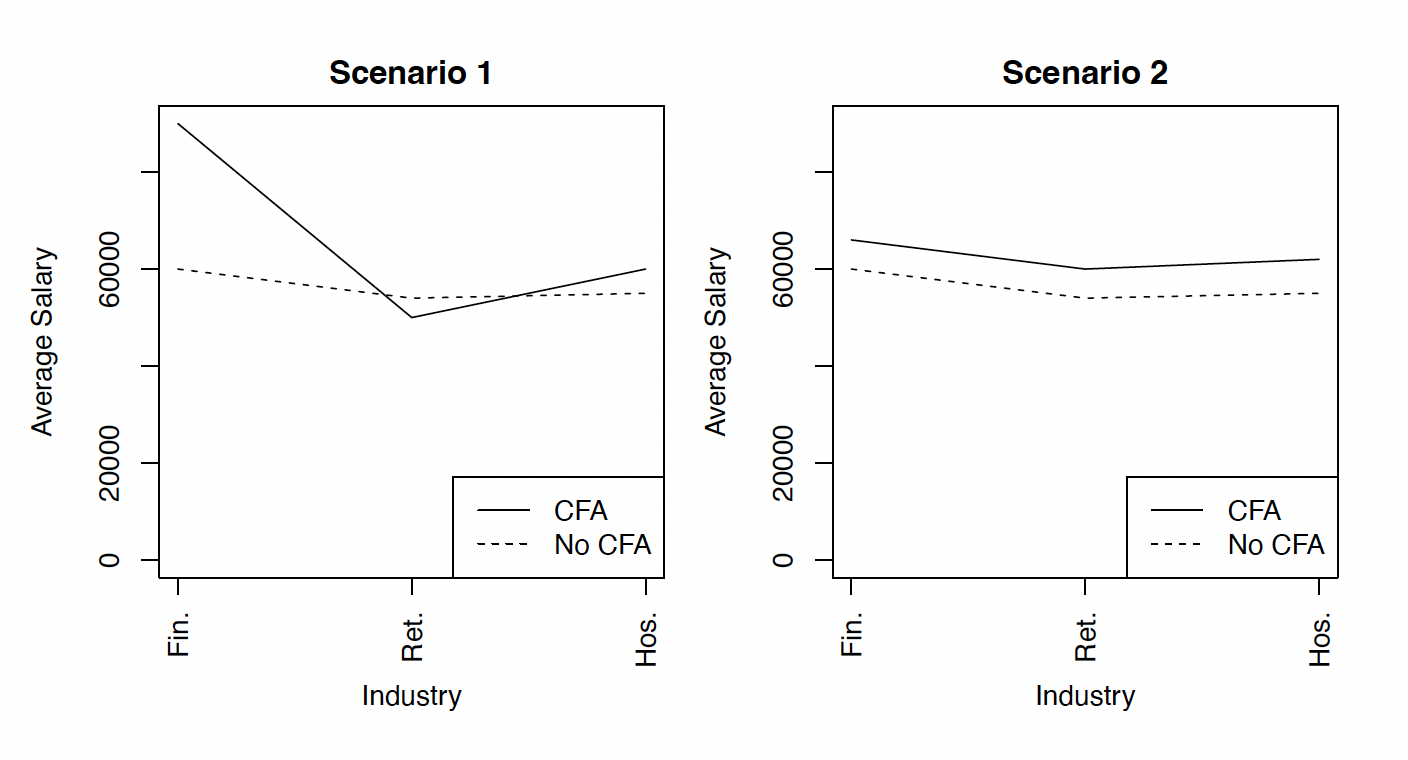
\includegraphics[width=12cm]{interaction.png}
	
	\end{frame}
\begin{frame}
	\frametitle{Interaction}
	
	\begin{itemize}[label={\color{blue}$\blacktriangleright$}]
		\item In scenario 1, the impact of having a CFA is most pronounced in the finance industry.
		
		\item In scenario 2, the impact of having a CFA is the same regardless of industry.
		
		\item We say that two factors \textbf{interact} when the effect of one factor on the response variable is altered by the level of the other factor.
		
		\item So there is an interaction between qualification and industry in scenario 1 but not in scenario 2.
	\end{itemize}
	
\end{frame}
\begin{frame}
	\frametitle{Interaction Hypotheses}
	
	\begin{itemize}[label={\color{blue}$\blacktriangleright$}]
		\item With a two-way ANOVA we can test whether an interaction exists between the factors:
		
		\vspace{0.3cm}
		$H_0$ : There is \textit{no interaction} between the factors.
		
		\vspace{0.2cm}
		$H_1$ : There is \textit{an interaction} between the factors.
		
		\item The interaction hypotheses should be tested first, before testing the \textit{main effects hypotheses}.
	\end{itemize}
	
\end{frame}
\begin{frame}
	\frametitle{Main Effects Hypotheses}
	
	\begin{itemize}[label={\color{blue}$\blacktriangleright$}]
		\item With a two-way ANOVA we can test the importance of each individual factor:
		
		\vspace{0.3cm}
		$H_0$ : The population means at different levels of the factor are all equal.
		
		\vspace{0.2cm}
		$H_1$ : At least two of the population means differ.
		
		\item If an interaction exists, the results of the main effects hypotheses should be interpreted carefully.
	\end{itemize}
	
\end{frame}
\begin{frame}
	\frametitle{Sums of Squares}
	
	\begin{itemize}[label={\color{blue}$\blacktriangleright$}]
		\item Suppose our two factors, denoted $A$ and $B$, have $a$ and $b$ levels, respectively, and we sample $r$ replicates in each treatment (i.e., $n = a \times b \times r$).
		
		\item We can calculate a sum of squares for factor $A$ ($SS_A$), for factor $B$ ($SS_B$), for the interaction ($SS_{AB}$), for the error ($SSE$) and also for the total ($SS(Total)$).
		
		\end{itemize}
	
\end{frame}
\begin{frame}
	\frametitle{Sums of Squares}
	
	\begin{itemize}[label={\color{blue}$\blacktriangleright$}]
		\item The sums of squares satisfy the following identity:
		
		\vspace{0.3cm}
		\[SS(Total) = SS_A + SS_B + SS_{AB} + SSE\]
		\vspace{0.3cm}
		
		\item The $SS(Total)$ again measures the total variation that exists in the data.
		
		\item The $SS_A$, $SS_B$ and $SS_{AB}$ measure how much variation can be explained by each particular source.
		
		\item The $SSE$ measures the left-over, unexplained variation.
	\end{itemize}
	
\end{frame}
\begin{frame}
	\frametitle{Test Statistics}
	
	\begin{itemize}[label={\color{blue}$\blacktriangleright$}]
		\item To test the interaction and main effects hypotheses, we need to see how big the $SS_{AB}$, $SS_A$ and $SS_B$ are, compared to the $SSE$.
		
		\item Again convert the sums of squares to mean squares, so that we can calculate $F$-statistics.
		
		\item The appropriate degrees of freedom, the mean squares and the $F$-statistics are listed in the ANOVA table shown next.
	\end{itemize}
	
\end{frame}
\begin{frame}
	\frametitle{ANOVA Table}
	\scriptsize
	
	\begin{center}
		\begin{tabular}{lcccc}
			\toprule
			\multirow{2}{*}{Source} & Sum of &Degrees of& Mean squares& $F$-statistic \\
			& squares & freedom &  &\\[1ex]
			\midrule
			Factor $A$ & $SS_A$ & $a-1$ & $MS_A = \frac{SS_A}{a-1}$ & $F_A = \frac{MS_A}{MSE}$ \\[1ex]
			Factor $B$ & $SS_B$ & $b-1$ & $MS_B = \frac{SS_B}{b-1}$ & $F_B = \frac{MS_B}{MSE}$ \\[1ex]
			Interaction & $SS_{AB}$ & $(a-1)(b-1)$ & $MS_{AB} = \frac{SS_{AB}}{(a-1)(b-1)}$ & $F_{AB} = \frac{MS_{AB}}{MSE}$ \\[1ex]
			Error & $SSE$ & $n-ab$ & $MSE = \frac{SSE}{n-ab}$ & \\[1ex]
			\midrule
			Total & $SS(Total)$ & $n-1$ & & \\[1ex]
			\bottomrule
		\end{tabular}
	\end{center}
	
\end{frame}
\begin{frame}
	\frametitle{ANOVA Table - Summary}
	
	\begin{itemize}[label={\color{blue}$\blacktriangleright$}]
		\item Degrees of freedom:
		\begin{itemize}[label={\color{blue}$\blacktriangleright$}]
			\item For a factor it is equal to the number of levels minus one.
			\item For the interaction it is equal to the product of the degrees of freedom of the two factors.
			\item All the degrees of freedom (excluding the total) will sum to $n-1$.
		\end{itemize}
		
		\item $F$-statistic:
		\begin{itemize}[label={\color{blue}$\blacktriangleright$}]
			\item Mean squares are calculated by dividing the sum of squares by the degrees of freedom.
			\item All $F$-statistics use the $MSE$ in the denominator.
		\end{itemize}
	\end{itemize}
	
\end{frame}
\begin{frame}
	\frametitle{Decision Rule}
	
	\begin{itemize}[label={\color{blue}$\blacktriangleright$}]
		\item We need to compare each $F$-statistic to an appropriate $F$-distribution.
		
		\item All hypotheses (interaction and main effects) are \textit{one-tailed}, and we reject $H_0$ if the $F$-statistic is too large.
		
		\item At a significance level of $\alpha$, we reject $H_0$ if $F > F_{\alpha,df,n-ab}$, where $df$ is the source degrees of freedom and $F_{\alpha,df,n-ab}$ is the critical value that cuts off $100\alpha\%$ in the upper tail of an $F$-distribution with $df$ numerator degrees of freedom and $n-ab$ denominator degrees of freedom.
	\end{itemize}
	
\end{frame}
\begin{frame}
	\frametitle{Airlines Rating Example}
	
	\begin{itemize}[label={\color{blue}$\blacktriangleright$}]
		\item Recall the previous example where twenty passengers, from each of three airlines, rated their experience on a 0 to 100 scale.
		
		\item Suppose that for each airline, half of the twenty passengers traveled in business class, while the remaining half traveled in economy class.
		
		\item We want to know:
		\begin{itemize}[label={\color{blue}$\blacktriangleright$}]
			\item Does perceived quality vary between airlines?
			\item Does perceived quality vary between traveling class?
			\item Does traveling class alter the differences between airlines in terms of perceived quality?
		\end{itemize}
	\end{itemize}
	
\end{frame}
\begin{frame}
	\frametitle{ANOVA Table}
		\small
	
	\begin{center}
		\begin{tabular}{lccccc}
			\toprule
			\multirow{2}{*}{Source}& Sum of & Deg. of & Mean & \multirow{2}{*}{$F$-statistic} & \multirow{2}{*}{$p$-value} \\
			& squares & freedom & squares &&\\
			\midrule
			\textcolor{red}{Airline} & 3446.80 & 2 & 1723.40 & \textcolor{red}{14.60} & \textcolor{red}{0.0000} \\
			\textcolor{red}{Class} & 6060.15 & 1 & 6060.15 & \textcolor{red}{51.34} & \textcolor{red}{0.0000} \\
			\textcolor{red}{Interaction} & 130.00 & 2 & 65.00 & \textcolor{red}{0.55} & \textcolor{red}{0.5798} \\
			Error & 6374.30 & 54 & 118.04 & & \\
			\midrule
			Total & 16011.25 & 59 & & & \\
			\bottomrule
		\end{tabular}
	\end{center}
	
\end{frame}
\begin{frame}
	\frametitle{Interaction}
	
	\begin{itemize}[label={\color{blue}$\blacktriangleright$}]
		\item Hypotheses:
		
		\vspace{0.3cm}
		$H_0$ : Airline and class do not interact.
		
		$H_1$ : Airline and class interact.
		
		\item From the output, we see that the $F$-statistic is 0.55 with a $p$-value of 0.5798.
		
		\item Since the $0.5798 > 0.05$, we fail to reject $H_0$ and we conclude that there is no interaction between airline and traveling class.
	\end{itemize}
	
\end{frame}
\begin{frame}
	\frametitle{Main Effects}
	
	\begin{itemize}[label={\color{blue}$\blacktriangleright$}]
		\item Hypotheses:
		\begin{align*}
			H_0 &: \text{Pop. mean ratings are equal between airlines.} \\
			H_1 &: \text{Pop. mean ratings differ between airlines.}
		\end{align*}
		
		\item From the output, we see that the $F$-statistic is 14.60 with a $p$-value of 0.0000.
		
		\item Since the $0.0000 < 0.05$, we reject $H_0$ and we conclude that perceived quality varies between airlines.
	\end{itemize}
	
\end{frame}
\begin{frame}
	\frametitle{Main Effects}
	
	\begin{itemize}[label={\color{blue}$\blacktriangleright$}]
		\item Hypotheses:
		\begin{align*}
			H_0 &: \text{Pop. mean ratings are equal between class.} \\
			H_1 &: \text{Pop. mean ratings differ between class.}
		\end{align*}
		
		\item From the output, we see that the $F$-statistic is 51.34 with a $p$-value of 0.0000.
		
		\item Since the $0.0000 < 0.05$, we reject $H_0$ and we conclude that perceived quality varies between travelling class.
	\end{itemize}
	
\end{frame}
\begin{frame}
	\frametitle{Airline Ratings ANOVA Tables}
	
	\begin{table}
		\small
		\begin{tabular}{llcccc}
			\toprule
			& Source & \begin{tabular}[c]{@{}c@{}}Sum of\\squares\end{tabular} & \begin{tabular}[c]{@{}c@{}}Deg. of\\freedom\end{tabular} & \begin{tabular}[c]{@{}c@{}}Mean\\squares\end{tabular} & $F$-statistic \\
			\midrule
			\multirow{3}{*}{\begin{tabular}[c]{@{}l@{}}One-way\\ANOVA\end{tabular}} 
			& Airline & 3446.8 & 2 & 1723.4 & 7.8184 \\
			& Error & 12564.45 & 57 & 220.4289 & \\
			\cline{2-6}
			& Total & 16011.25 & 59 & & \\
			\bottomrule
			\multirow{5}{*}{\begin{tabular}[c]{@{}l@{}}Two-way\\ANOVA\end{tabular}} 
			& Airline & 3446.80 & 2 & 1723.40 & 14.60 \\
			& Class & 6060.15 & 1 & 6060.15 & 51.34 \\
			& Interaction & 130.00 & 2 & 65.00 & 0.55 \\
			& Error & 6374.30 & 54 & 118.04 & \\
			\cline{2-6}
			& Total & 16011.25 & 59 & & \\
			\bottomrule
		\end{tabular}
	\end{table}
	
\end{frame}
\begin{frame}
	\frametitle{One-way and Two-way ANOVA}
	
	\begin{itemize}[label={\color{blue}$\blacktriangleright$}]
		\item Suppose we perform both a one-way ANOVA and a two-way ANOVA, using a \emph{balanced design}, on the \emph{same} data with a factor in common.
		\begin{itemize}[label={\color{blue}$\blacktriangleright$}]
			\item The $SS(\text{Total})$ will be the same for both.
			\item The $SST$ in the one-way ANOVA will be the same as the sum of squares for the corresponding factor in the two-way ANOVA.
			\item The two-way ANOVA accounts for more variation than the one-way ANOVA.
			\item This means that for the two-way ANOVA, there is \emph{less} unexplained variation so the $SSE$ will be smaller than for the one-way ANOVA.
		\end{itemize}
	\end{itemize}
	
\end{frame}
\end{document}